\chapauthor{Василевская А.П.\\Орлов М.К.\\Шункевич Д.В.}
\chapter{Логические, продукционные и функциональные модели решения задач в ostis-системах}
\chapauthortoc{Василевская А.П.\\Орлов М.К.\\Шункевич Д.В.}
\label{chapter_logic_productions}

\abstract{Аннотация к главе.}

\section{Операционная семантика логических языков, используемых ostis-системами}

% Назвать подходы в ИИ. Место логики в ИИ

Логика решает задачи доказательства истинности высказываний, аргументации того или иного высказывания, задачу генерации и опровержения гипотез. Некоторые гипотезы могут быть опровергнуты, однако извлекая причины того, почему гипотеза опровергнута, можно изменить посылку гипотезы так, чтобы создать новую гипотезу, которая впоследствии может стать теоремой.

Современная логика изучает формальные языки, служащие для выражения логических рассуждений.
Логический язык -- искусственный язык логики, предназначенный для воспроизведения логических форм контекстов естественного языка, а также выражения логических законов и способов правильных рассуждений в логических теориях, строящихся в данном языке. Логика не изучает то, как были получены знания, она позволяет из существующих знаний вывести новые (точнее из имеющихся формул логики вывести новые формулы этой же логики), установить правильность рассуждений. Получение новых формул логики на основе существующих осуществляется логическим выводом.

% [Коротков, Степанов - Основы формальных логических языков, 2003]
Правильность умозаключений вводится и проверяется совершенно формально, без какой-либо связи с истинностью входящих в него посылок, т.е. исключительно с точки зрения структуры рассуждения. С практической точки зрения самое важное свойство такой формальной правильности рассуждений заключается в следующем: если нам удалось доказать, пользуясь методами формальной логики, правильность рассуждения, и нам известно из опыта, что все используемые посылки истинны, то мы можем быть уверены в истинности заключения. Истинность используемых посылок трактуется фактом принадлежности этих посылок формальной теории, в которой происходит логический вывод, то есть задаётся состоянием базы знаний.

База знаний интеллектуальной системы включает в себя как модель фактографических знаний о предметной области, для которой предназначена система, так и модель знаний, включающая в себя логические формулы об этой предметной области (аксиомы, теоремы и правила вывода).

% Отсебятина
В логике выделяют два подхода: содержательный и формальный подход. В содержательном подходе используются истинностные таблицы для анализа логической формулы. Формальный подход основывается на понятии логического вывода без интерпретации таблиц истинности. Для вычисления истинностных таблиц существует тривиальный алгоритм, однако при большом количестве переменных и подформул этот метод является неэффективным. В свою очередь при формальном подходе решение может быть более изящным (коротким), но не очевидно, какую аксиому применить и с какими значениями переменных этой аксиомы с тем или иным правилом вывода.

% Обосновать крепче
В связи с этим больший практический и научный интерес представляет формальный подход.

% Вагин, дедукция и обобщение в системах принятия решений
Выводом в формальной системе называется любая последовательность формул такая, что любая формула либо аксиома этой формальной системы, либо непосредственное следствие каких-либо предыдущих формул по одному из правил вывода.
Идея выводимости центральна в логике: в любой формальной аксиоматической теории `теорема' – это формула, которая выводится из аксиом.
Формула F (логически) следует из множества формул G (или множество формул G влечёт формулу F, символически, G |= F ), если для каждой интерпретации, при которой все формулы G истинны, формула F также истинна. В то же время с точки зрения формального подхода G влечёт F, если F может быть выведено из G с использованием определенного набора ``правил вывода''.

% Семантические сети в логическом выводе
% Вагин, дедукция и обобщение в системах принятия решений, стр 32
Семантические сети удобны для представления знаний любого вида, в том числе логических формул. Применение семантических сетей для дедуктивного вывода исследовалось Квиллианом в 1966. Он формально представлял семантику слов естественного языка и дал несколько примеров техники вывода, основанной на поиске по пересечению с использованием распространения активности. Дедуктивные возможности Квиллиана фактически определялись понятием "подкласс" и отношением "модификации". Понятие может быть определено в терминах более общего понятия и с помощью модифицирующего свойства, которое является комбинацией атрибут - значение атрибута.
Важной техникой, используемой в семантических сетях, является иерархия или система классификации. В соответствии с этой техникой объекты, относящиеся к предметной области, классифицируются на некоторое число категорий или классов на основании их общих свойств. Используя иерархическую систему в богатой базе знаний интеллектуальной системы, особенно выгодно (удобно) использовать логический вывод, ведь тот вывод, который справедлив для общих понятий будет справедливым и для частных понятий по отношению к этому общему. Такая схема рассуждений описывается известным силлогизмом "если для Б справедливо В и А есть Б, то В справедливо и для А". 
% Ниже можно посмотреть Г. Хендрикс (очерчивание). Возможное преимущество нашего подхода -- мы не используем базу данных отдельно от семантической сети для хранения утверждений и правил, нету также словаря семантических категорий
Другой важной техникой, используемой в логическом выводе на семантических сетях является локализация знаний. Суть локализации в том, что можно выделить область (структуру) семантической сети, в которой находятся предметные знания (константы, например, экземпляры классов), пригодные для использования в посылках логического вывода. Учитывая иерархичность базы знаний становится наиболее удобно выделить универсум рассуждений, выходить за который не целесообразно. Таким образом область значений переменных, находящихся в посылках логических формул ограничена, что позволяет существенно сократить затраты на поиск в больших базах знаний. 
Переменные представляют собой свободные и связанные предметные переменные, которые являются интенсиональными объектами и ассоциируются (имеют значение) с некоторым одним константным элементом из базы знаний. 
В особых случаях можно разграничивать области рассуждений от более узких и в то же время наиболее вероятных для достижения результата логического вывода до более широких областей, сущности которых менее вероятно будут использованы в логическом выводе, постепенно объединяя эти области поиска в случае не достижения цели логического вывода сразу в первоначальной области.

% Отсебятина
Главное преимущество использования SC-кода для формализации и обработки логических формул в том, что он обеспечивает совместимость между различными моделями решения задач. Любая ostis-система имеет решатель задач и бывают задачи, для которых заранее неизвестен алгоритм их решения, нету готового метода. Система должна думать и определять, какие агенты могут быть привлечены для решения той или иной задачи.

Формализм SC-кода позволяет описывать отношения между понятиями любой формы и сложности, что делает его подходящим вариантом для использования логического вывода в интеллектуальных компьютерных системах нового поколения. А также воспользоваться техникой иерархии за счёт онтологического подхода, лежащего в основе баз знаний ostis-систем.

% Источник этого текста и используемых в нём ссылок здесь https://libeldoc.bsuir.by/bitstream/123456789/30629/1/Golenkov_Grapho.pdf
SCL — подъязык SC-кода для записи логических утверждений. Язык SCL является логическим языком графового типа, используемым ostis-системами, тексты языка SCL представляют собой однородные семантические сети, являющиеся текстами языка SC [2]. Алфавит языка SCL отдельно не выделяется, так как используется алфавит SC-кода, на котором можно описать любые утверждения, явления, закономерности, программы и любые другие знания. Язык SCL позволяет записывать тексты языка логики высказываний, языка логики предикатов и любых других логических языков. SC-код является метаязыком как для языка SCL, так и для самого себя, то есть он позволяет описывать смысл формул, записанных на SCL. Многие формальные языки, в отличие от SC, недостаточно богаты, чтобы быть метаязыком для самих себя. Специфика выделения языка SCL в том, что тексты этого языка могут обрабатываться особым образом. Над формулами языка SCL можно проводить логический вывод.

Атомарная формула языка SCL трактуется как множество всех символов некоторого sc-текста (sc-структура). Каждая неатомарная формула языка SCL трактуется как связка, принадлежащая отношению, соответствующему типу неатомарной формулы (конъюнкция, дизъюнкция, отрицание, импликация, эквиваленция, существование, всеобщность) и связывающая знаки формул, входящих в состав указанной неатомарной формулы. Для формализации логических высказываний используется \textbf{\textit{Предметная область и онтология логических формул и высказываний}}.

Абстрактная scl-машина [9, 10, 11] является машиной логического вывода и относится к классу абстрактных sc-машин. Внутренним языком scl-машины является указанный выше графовый логический язык SCL, ее операции соответствуют правилам логического вывода [10,11]. Семейство специализированных абстрактных графодинамических машин обработки знаний является формальным уточнением операционной семантики указанных выше специализированных графовых языков представления знаний, каждому из которых соответствует одна или несколько абстрактных машин. Эти абстрактные машины соответствуют различным моделям решения задач, различным логикам, различным моделям правдоподобных рассуждений [12]. 
Агент из семейства агентов логического вывода может представлять собой какое-либо правило вывода, которое можно применять для решения задачи. Кроме того необходимы агенты для выполнения равносильных преобразований логической формулы (например, записать формулу эквиваленции как конъюнкцию двух дизъюнкций) и другие агенты, помогающие применять правила вывода на множестве формул языка логики.

% Кванторы по умолчанию
% Что значит изящной?
Одной из важных особенностей SCL является его способность изящной обработки и представления текстов языка логики предикатов. Язык SCL естественным образом ориентирован на работу в формальной системе языка логики предикатов. Язык SC позволяет записать любые отношения и соответствия в графовом представлении. Значению предиката от некоторого набора sc-переменных соответствует результат операции поиска по шаблону некоторой sc-конструкции (найдена или не найдена), в которую входят sc-константы и/или sc-переменные с соответствующей конфигурацией связей между ними. Подход, основанный на семантических сетях для представления формул и баз знаний для их хранения предоставляет возможность явно не записывать кванторы общности и существования (это не запрещается, однако является излишним). Квантор существования является "встроенным" понятием в том смысле, что если некоторый sc-элемент входит в некоторую sc-структуру, то соответствующее понятие существует в этой sc-структуре. Таким образом, квантор существования накладывается автоматически (если иной квантор не наложен явно) на те sc-переменные, которые входят в атомарные логические формулы. Квантор всеобщности накладывается по умолчанию (если иной квантор не наложен явно) на переменные, входящие в связки эквиваленции и импликации в соответствии с денотационной семантикой логических языков.

Такие особенности упрощают логический вывод в логике предикатов на языке SCL, так как избавляет от необходимости приводить высказывание в Сколемовскую нормальную форму за счёт встроенных кванторов и от необходимости процедуры унификации за счёт операции поиска sc-конструкции по шаблону, в которой проиходят необходимые подстановки переменных.

Различные логические подходы позволяют проектировать решатели задач для интеллектуальных систем в разных предметных областях, учитывая их специфику.
Машина обработки знаний каждой конкретной системы во многом зависит от назначения данной системы, множества решаемых задач, предметной областью и другими факторами. Некоторые операции, необходимые в одной предметной области будут избыточными в другой. Например, в системе, решающей задачи по геометрии, химии и другим естественным наукам обоснованным будет использование дедуктивных методов вывода, поскольку решение задач в таких предметных областях основывается только на достоверных правилах. В системах же медицинской диагностики, к примеру, постоянно возникает ситуация, когда диагноз может быть поставлен только с некоторой долей уверенности и абсолютно достоверным ответ на поставленный вопрос быть не может. В связи с этим возникает необходимость использования различных машин обработки знаний в различных системах, при этом состав и возможности машины обработки знаний в конкретной системе определяется не только непосредственно разработчиком, а требует консультаций с экспертами в данной предметной области.

\textbf{Агенты логического вывода}. К данному классу относятся агенты, предназначенные для генерации новых знаний на основе некоторых логических утверждений. Количество и разнообразие таких агентов зависит от типологии логических утверждений, которые предполагается использовать в прикладной интеллектуальной системе.

Проблема автоматического решения задач достаточно давно рассматривается в работах по искусственному интеллекту. Приведем краткую классификацию существующих логических методов решения задач:
\begin{itemize}
	\item{\textbf{Классический дедуктивный вывод.} Классический дедуктивный вывод является наиболее популярным при построении автоматических решателей задач, так как всегда дает достоверный результат. Дедуктивный вывод включает в себя прямой и обратный и логический вывод (принцип резолюции, процедуру Эрбрана и др.) [Вагин и др., 2008], все виды силлогизмов [Малыхина, 2002] и т.д. Основной проблемой
	дедуктивного вывода является невозможность его использования в ряде случаев, когда отсутствуют
	достоверные правила вывода.}
	\item{\textbf{Индуктивный вывод.} Индуктивный вывод предоставляет возможность в процессе решения использовать различные предположения, что делает его удобным для использования в слабоформализованных и
	трудноформализуемых предметных областях, например при построении систем медицинской диагностики. Подробно принципы индуктивного вывода рассмотрены в [Кулик, 2001], [Пойа, 1975].}
	\item{\textbf{Абдуктивный вывод.} Под абдуктивным выводом в искусственном интеллекте, как правило, понимается вывод наилучшего абдуктивного объяснения, т.е. объяснения некоторого события, ставшего
	неожиданным для системы. Причем «наилучшим»	считается такое объяснение, которое удовлетворяет специальным критериям, определяемым в зависимости от решаемой задачи и используемой	формализации. Абдуктивный вывод подробно рассматривается в [Вагин и др., 2008].}
	\item{\textbf{Нечеткие логики.} Теория нечетких множеств и, соответственно, нечетких логик, также применяется в системах, связанных с трудноформализуемыми предметными областями. Подробнее теория нечетких логик рассматривается в [Поспелов, 1989], [Батыршин, 2001], [Деменков, 2001] и других изданиях.}
	\item{\textbf{Логика умолчаний.} Логика умолчаний применяется, в том числе, для того, чтобы оптимизировать процесс рассуждений,	дополняя процесс достоверного вывода вероятностными  предположениями в тех случаях, когда вероятность ошибки крайне мала. Подробнее логика умолчаний рассмотрена в статье [RRIAI, 2012].}
	\item{\textbf{Темпоральная логика.} Применение темпоральной логики является очень актуальным для нестатичных предметных областей, в которых истинность того или иного утверждения меняется со временем, что существенно влияет на ход решения какой-либо задачи. Следует отметить, что используемый в 		данной работе язык представления знаний предоставляет все необходимые возможности для описания таких динамических предметных областей. Более подробно темпоральная логика рассмотрена в работе [Еремеев, 1997]}
\end{itemize}

% Вставить в статью
Данная работа не ставит своей целью разработку нового метода решения задач, нового класса логик или отрицание существующих достижений в данной области. Целью работы является разработка технологии, позволяющей интегрировать любые модели решения задач и принципы логического вывода для решения задач в интеллектуальных системах на основе общей формальной модели. Для того, чтобы использовать какую-либо новую или существующую модель, необходимо привести ее предлагаемому в данной работе формализму, что позволить интегрировать и синхронизировать ее с уже имеющимися в соответствующей библиотеке совместимых компонентов.

\begin{SCn}
	\scnheader{Семейство агентов логического вывода}
	\begin{scneqtoset}
		\scnitem{Агент прямого логического вывода}
		\scnitem{Агент обратного логического вывода}
		\scnitem{Агент применения правила вывода}
		\scnitem{Агент эквиалентных преобразований логической формулы}
		\begin{scnindent}
			\begin{scnrelfromset}{разбиение}
				\scnitem{Агент применения законов Де Моргана}
				\scnitem{Агент преобразования формулы в конъюнктивную нормальную форму}
				\scnitem{Агент преобразования формулы в дизъюнктивную нормальную форму}
				\scnitem{Агент эквиалентных преобразований логической формулы по определению} % ???
				\scnitem{Агент применения законов равносильных преобразований логических формул}
				\begin{scnindent}
					\begin{scnrelfromset}{разбиение}
						\scnitem{Агент применения закона идемпотентности логических формул}
						\scnitem{Агент применения закона коммутативности логических формул}
						\scnitem{Агент применения закона ассоциативности логических формул}
						\scnitem{Агент применения закона поглощения логических формул}
						\scnitem{Агент применения закона противоречия логических формул}
						\scnitem{Агент применения закона двойного отрицания логических формул}
						\scnitem{Агент применения закона расщепления логических формул}
					\end{scnrelfromset}
				\end{scnindent}
			\end{scnrelfromset}
		\end{scnindent}
	\end{scneqtoset}
\end{SCn}

Также можно использовать стратегии решения задач путём упрощения задачи (переход от формулировки в терминах предметной области к формулировке на логическом языке):
\begin{itemize}
	\item{операция обобщения;}
	\item{вывод обобщенного логического высказывания;}
	\item{фаззификация;}
	\item{дефаззификация;}
	\item{применение аналогий;}
	\item{и другие.}
\end{itemize}

Применение аналогий:
\begin{itemize}
	\item{генерация логического утверждения по аналогии;}
	\item{восстановление решения после применения аналогии;}
	\item{генерация фактов по аналогии;}
	\item{и другие.}
\end{itemize}

Используя такие агенты можно решать следующие задачи:
\begin{itemize}
	\item{генерация знаний на основании определения (эквиваленции)}
	\item{генерация определения (эквиваленции) на основании двух импликаций}
	\item{получение значения некоторой продукции}
	\item{вывод обобщенного высказывания}
	\item{генерация связки отношения на основании логического утверждения}
\end{itemize}
% Я не знаю что это
% \item{получение значения некоторой продукции;}
% \item{Агент генерации связки отношения на основании логического утверждения}

Генерация всех возможных следствий (прямой логический вывод):
\begin{itemize}
	\item{поиск всех возможных правил для применения;}
	\item{применение найденных правил;}
	\item{проверка новых фактов на то, что они отсутствуют в базе знаний;}
	\item{дополнение базы знаний сгенерированными фактами;}
	\item{восстановление решения;}
	\item{и другие.}
\end{itemize}

% А где шаблон того, что мы хотим получить в результате?
Под операцией логического вывода понимается некоторый sc-агент, который получает на вход теоретико-множественную пару {S, O}, где S - логическое утверждение произвольной конфигурации, O - совокупность объектов, в семантической окрестности которых необходимо применить утверждение S. Целью такого агента является генерация в памяти новых знаний на основании уже имеющихся, т.е. по сути, применение утверждения S. Указанный процесс поиска ответа можно разделить на следующие этапы:

\begin{itemize}
	\item{\textbf{Этап работы поисковых операций.} Вне зависимости от типа поставленного вопроса всегда имеется вероятность того, что данная задача уже была решена системой ранее или системе уже 	откуда-либо известен ответ на поставленный вопрос. На данном этапе работу осуществляет коллектив поисковых операций, каждая из которых, как правило, соответствует некоторому классу	решаемых задач. Если ответ найден, подсистема обработки знаний прекращает свою работу. В противном случае происходит переход на следующий этап решения.}
	\item{\textbf{Этап применения стратегий решения задач.}	На данном этапе осуществляется выбор между
	различными стратегиями решения задач, и, при необходимости, параллельный запуск различных стратегий. Целью работы каждой из стратегий является получение набора пар, связывающих некоторое множество объектов и логическое утверждение из базы знаний, которое справедливо для классов, которым принадлежат эти объекты в рамках некоторой теории. Впоследствии при	рассмотрении каждого утверждения осуществляется	попытка применить его в рамках некоторой семантической окрестности рассматриваемых объектов, для чего осуществляется переход на следующий этап решения.}
	\item{\textbf{Этап применения правил логического вывода.} На данном этапе происходит попытка применения утверждения, полученного на предыдущем шаге, с целью генерации в системе	новых знаний. Если такое применение справедливо (например, посылка истинна) и имеет смысл (в результате применения будут сгенерированы новые знания), то осуществляется генерация новых знаний на основе одного из правил логического вывода. При этом применение происходит в контексте объекта, рассматриваемого на предыдущем этапе (в общем случае – ряда объектов). Если в данном контексте вывод на основе данного утверждения	невозможен или нецелесообразен, решение возвращается на предыдущий этап. В случае успешного применения утверждения происходит переход к следующему этапу решения.}
	\item{\textbf{Этап верификации и оптимизации сгенерированных знаний и сборки мусора.} На данном этапе происходит интерпретация арифметических отношений, сгенерированных в процессе решения на предыдущем этапе, то есть попытка вычисления недостающих значений компонентов связок арифметических отношений
	(например, сложение величин и произведение величин) на основе имеющихся значений. Если вычислить все недостающие значения не представляется возможным, то все знания, сгенерированные на предыдущем этапе,
	уничтожаются и решение переходит на этап применения стратегий. В таком случае применение логического вывода для рассматриваемого на предыдущем шаге утверждения считается не	целесообразным. Также на данном этапе происходит устранение синонимии, если таковая появилась на предыдущем этапе решения,
	например, сгенерирована связка отношения совпадения между некоторыми объектами. В конечном итоге происходит удаление конструкций, ставших ненужными и по каким-либо причинам не удаленных на предыдущих этапах решения. Если все этапы решения выполнены успешно, то решение возвращается к первому этапу, и в случае, если ответ не получен, процесс повторяется еще раз. Стоит отметить, что в процессе решения один и тот же объект или одно и тоже высказывание могут быть использованы многократно, если это целесообразно. Однако, очевидно, что применение одного и того же утверждения для одного объекта несколько раз не имеет смысла, при условии, что нужные знания из памяти не удаляются в процессе решения какими-либо сторонними операциями. Следует учитывать тот факт, что агенты сборки мусора, устранения синонимии и верификации знаний могут оказаться полезными и необходимыми не только на завершающем этапе работы интеллектуального решателя задач. В этом смысле 4-ый этап может быть частично интегрирован с какими-либо из предыдущих.}
\end{itemize}

Таким образом, в структуре описываемой модели можно выделить 4 логических уровня, на каждом из которых возможно использование методов параллельной обработки информации. 

\begin{figure}[H]
	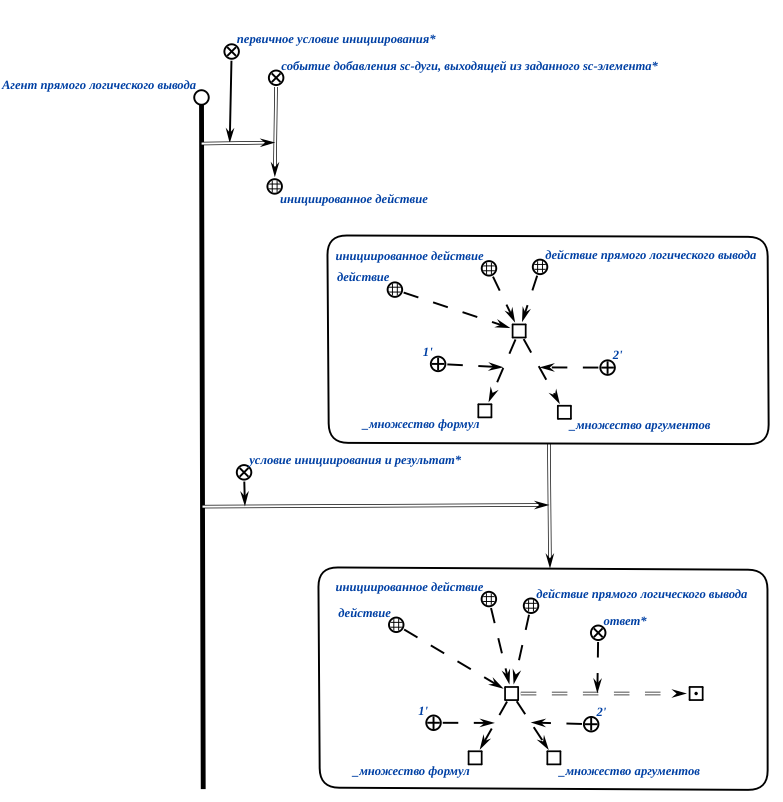
\includegraphics[scale=0.8]{author/part3/figures/direct_inference_agent.png}
	\caption{Спецификация агента прямого логического вывода}
	\label{fig:direct_inference_agent}
\end{figure}

\begin{figure}[H]
	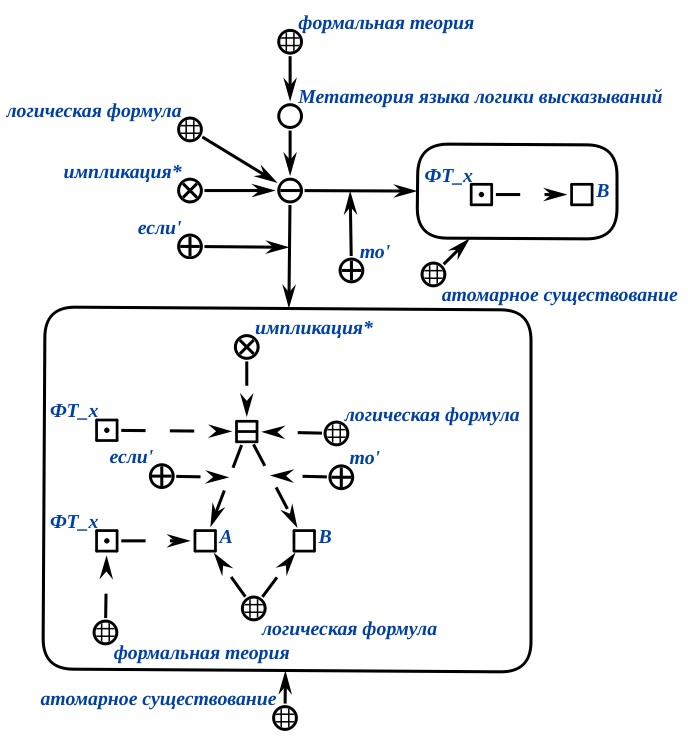
\includegraphics[scale=0.8]{author/part3/figures/Modus_ponens.png}
	\caption{Формализация правила вывода Modus ponens}
	\label{fig:modus_ponens}
\end{figure}

% Специфицировать агентно
Любая формула эквивалентна некоторой формуле в конъюнктивной нормальной форме, в связи с этим иногда удобно применять правило резолюции. Также любая ostis-система должна уметь учитывать НЕ-факторы знаний. Используя законы Де Моргана можно также получить формулы, пригодные для использования правила резолюции.
С помощью правила резолюции можно эффективно доказывать формулы языка логики высказываний.
% Это вообще под вопросом
Применение правила резолюции проще, чем использование правила Modus ponens с аксиомами, потому что не нужно выбирать нужную аксиому и значения для переменных этой аксиомы, а только применять правило резолюции столько раз, сколько потребуется.
Применение правила резолюции проще, чем использование правила Modus ponens с аксиомами, потому что не нужно выбирать нужную аксиому и значения для переменных этой аксиомы, а только применять правило резолюции столько раз, сколько потребуется.
Однако ничего принципиально нового правильно резолюции не привносит, поскольку формула $A \Rightarrow B$  равносильно $\neg A \lor B$ и из выводимости A и $A \rightarrow B$ следует выводимость B.

\begin{figure}[H]
	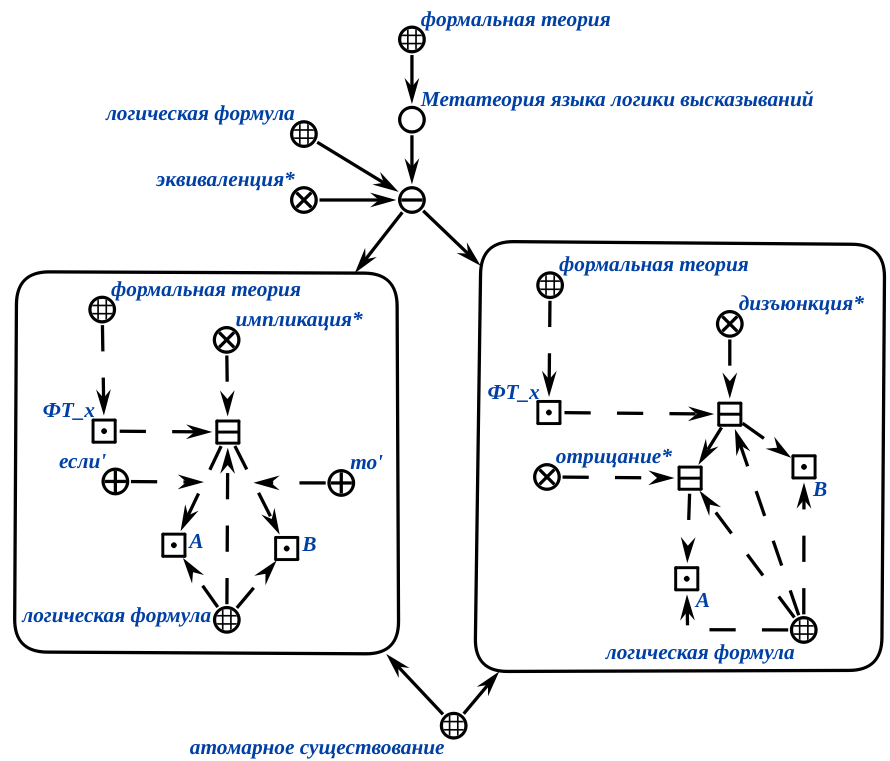
\includegraphics[scale=0.8]{author/part3/figures/conjunction_implication_rule.png}
	\caption{Формализация конъюнктивной нормальной формы для импликации}
	\label{fig:conjunction_implication_rule}
\end{figure}

Если в любых двух дизъюнктах $C_1$ и $C_2$ имеется пара формул $A$ и $\not A$, то можно сформировать новый дизъюнкт из оставшихся частей изначальных дизъюнктов.

\begin{figure}[H]
	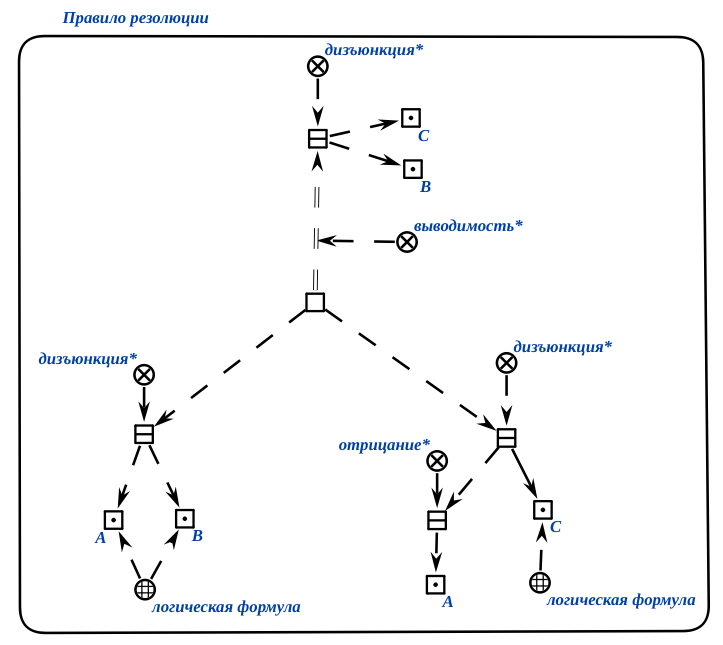
\includegraphics[scale=0.8]{author/part3/figures/resolution.png}
	\caption{Формализация правила резолюции}
	\label{fig:resolution}
\end{figure}

Приведём пример вывода формулы из множества посылок принципом резолюции.
Если команда A выигрывает в футбол, то город A' торжествует, а если выигрывает команда B, то торжествовать будет город B'. Выиграть может или только город A', или только город B'. Однако, если выигрывает команда A, то город B' не торжествует, а если выигрывает команда B, то не торжествует город A'. Следовательно, город B' торжествует тогда и только тогда, когда не будет торжествовать город A'. Цель логического вывода - удостовериться, что город B' торжествует тогда и только тогда, когда не будет торжествовать город A'. Доказать вывода формулы равносильно доказательству противоречивости вывода отрицания этой формулы. При использовании правила резолюции это особенно удобно использовать.
Формализация логических формул, соответствующих примеру приведена на рисунке ниже. Каждая неатомарная формула на рисунке принадлежит некоторой формальной, то есть считается истинной.

\begin{figure}[H]
	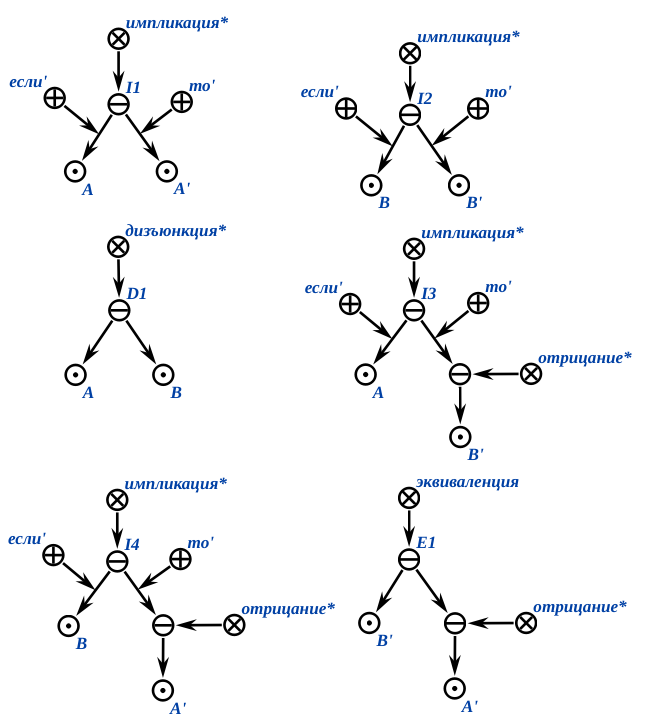
\includegraphics[scale=0.8]{author/part3/figures/resolution_formulas_example.png}
	\caption{Формализация правил для применения правила резолюции}
	\label{fig:resolution_formulas}
\end{figure}

Структура A представляет собой атомарную логическую формулу, которая обозначает победу команды A, структура A' представляет формулу, обозначающую торжество города A'. Соответственно, то же самое для структур B и B'.
Прежде всего необходимо привести импликацию в конъюнктивную нормальную форму по формуле \ref{fig:conjunction_implication_rule} и эквиваленцию по определению. А также применим отрицание к формуле, которую необходимо вывести (эвиваленция). В результате получим следующие формулы:

\begin{figure}[H]
	\includegraphics[scale=0.8]{author/part3/figures/resolution_prepared_formulas_example.png}
	\caption{Формализация правил для применения правила резолюции после преобразования в конъюнктивную нормальную форму}
	\label{fig:resolution_formulas}
\end{figure}

Далее применяя правило резолюции для преобразованных формул получаем пустой дизъюнкт, что говорит о противоречивости множества формул и доказывает формулу эквиваленции о том, что город B' торжествует тогда и только тогда, когда не будет торжествовать город A'.

\begin{figure}[H]
	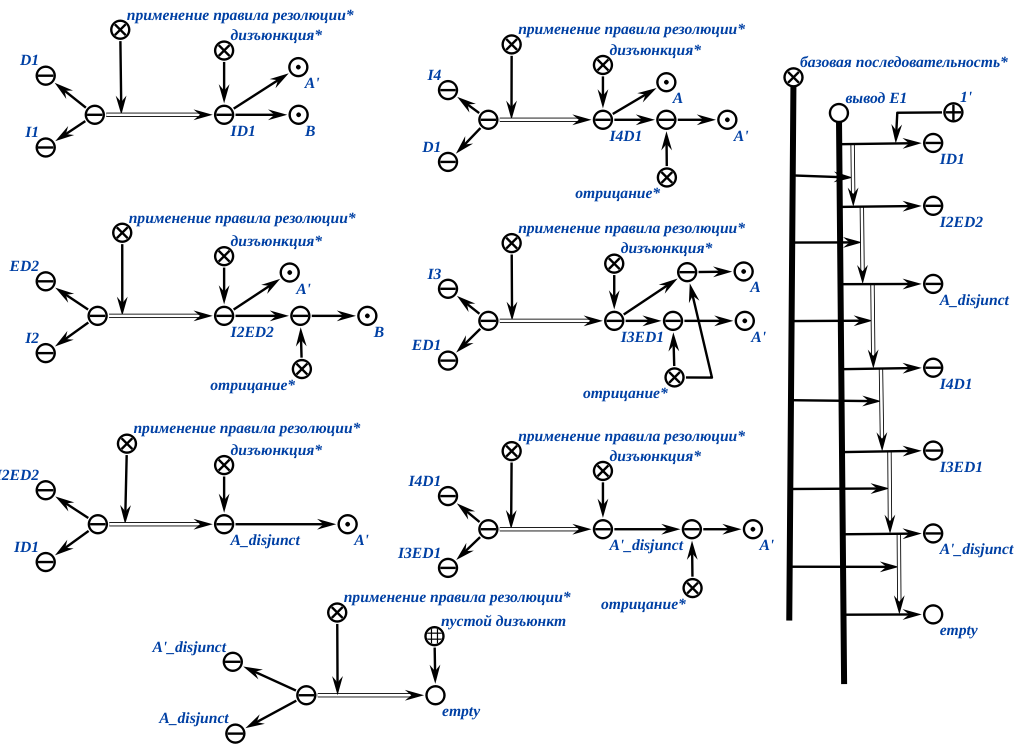
\includegraphics[scale=0.7]{author/part3/figures/resolution_inference.png}
	\caption{Применение принципа резолюции}
	\label{fig:resolution_inference}
\end{figure}

% Привести сравнение формального вывода этой же формулы через MP и аксиомные схемы, сделать сравнение

\section{Языки продукционного программирования, используемые ostis-системами}
\subsection{Синтаксис языков продукционного программирования, используемых ostis-системами}
\subsection{Денотационная семантика языков продукционного программирования, используемых ostis-системами}
\subsection{Операционная семантика языков продукционного программирования, используемых ostis-системами}

%\input{author/references}